%%%%%%%%%%%%%%%%%%%%%%%%%%%%%%%%%%%%%%%%%%%%%%%%%%%%%%%%%%%%%%%%%%%%
%% I, the copyright holder of this work, release this work into the
%% public domain. This applies worldwide. In some countries this may
%% not be legally possible; if so: I grant anyone the right to use
%% this work for any purpose, without any conditions, unless such
%% conditions are required by law.
%%%%%%%%%%%%%%%%%%%%%%%%%%%%%%%%%%%%%%%%%%%%%%%%%%%%%%%%%%%%%%%%%%%%

\documentclass{beamer}
\usetheme[faculty=ped]{fibeamer}
\usepackage[utf8]{inputenc}
\usepackage{lastpage}
\usepackage[
  main=english, %% By using `czech` or `slovak` as the main locale
                %% instead of `english`, you can typeset the
                %% presentation in either Czech or Slovak,
                %% respectively.
  czech, slovak %% The additional keys allow foreign texts to be
]{babel}        %% typeset as follows:
%%
%%   \begin{otherlanguage}{czech}   ... \end{otherlanguage}
%%   \begin{otherlanguage}{slovak}  ... \end{otherlanguage}
%%
%% These macros specify information about the presentation

  %-------------------------------------------------------------------------------
\newcommand{\mrm}{Marcelo de Rezende Martins} % Prénom et Nom Auteur 1
\newcommand{\magerosa}{Marco Aurélio Gerosa} % Prénom et Nom Auteur 1 (version courte pied de page)

\title{CoNCRA: A Convolutional Neural Network Code Retrieval Approach} %% that will be typeset on the
\subtitle{XXXIV Brazilian Symposium on Software Engineering} %% title page.
\author[\mrm \ \textit{et al.}]{\mrm\inst{1}, \magerosa\inst{2}}
\date[23/10/2020]{October 23, 2020}
\institute{
 \par \inst{1} Institute for Technological Research (IPT)
 \par \inst{2} Northern Arizona University (NAU)
 }
  
  \setbeamertemplate{footline}[text line]{%
  \parbox{\linewidth}{\vspace*{-8pt}SBES 2020\hfill De Rezende Martins and Gerosa \hfill\thepage\hspace{0.05cm}/ \pageref{LastPage}}}

%-------------------------------------------------------------------------------
  
  % BEGIN OF CODE POSTED AT SO
\RequirePackage{ifthen} % package required

\newboolean{sectiontoc}
\setboolean{sectiontoc}{true} % default to true

\AtBeginSection[]
{
  \ifthenelse{\boolean{sectiontoc}}{
    \begin{frame}<beamer>{Gliederung}
      \tableofcontents[currentsection]
    \end{frame}
  }
}

\newcommand{\toclesssection}[1]{
  \setboolean{sectiontoc}{false}
  \section{#1}
  \setboolean{sectiontoc}{true}
}
% END OF CODE POSTED AT SO
  
  
 \makeatletter
\setbeamertemplate{title page}{%
  % This is slide 0
  \setcounter{framenumber}{0}

  % Input the university logo
  \begin{tikzpicture}[
    remember picture,
    overlay,
    xshift=0.5\fibeamer@lengths@logowidth,
    yshift=0.5\fibeamer@lengths@logoheight
  ]
    \node at (0,0) {
      \fibeamer@includeLogo[
        width=\fibeamer@lengths@logowidth,
        height=\fibeamer@lengths@logoheight
      ]};
  \end{tikzpicture}

  % Input the title
  \usebeamerfont{title}%
  \usebeamercolor[fg]{title}%
  \begin{minipage}[b][2\baselineskip][b]{\textwidth}%
    \raggedright\inserttitle
  \end{minipage}
  \vskip-.5\baselineskip

  % Input the dashed line
  \begin{pgfpicture}
    \pgfsetlinewidth{2pt}
    \pgfsetroundcap
    \pgfsetdash{{0pt}{4pt}}{0cm}

    \pgfpathmoveto{\pgfpoint{0mm}{0mm}}
    \pgfpathlineto{\pgfpoint{\textwidth}{0mm}}

    \pgfusepath{stroke}
  \end{pgfpicture}
  \vfill
  % Input the subtitle
  \usebeamerfont{subtitle}%
  \usebeamercolor[fg]{subtitle}%
  \begin{minipage}{\textwidth}
    \raggedright%
    \insertsubtitle%
  \end{minipage}\vskip.25\baselineskip

  % Input the author's name
  \usebeamerfont{author}%
  \usebeamercolor[fg]{author}%
  \begin{minipage}{\textwidth}
    \raggedright%
    \insertauthor\newline%
    \par \insertdate\newline%
    \tiny\insertinstitute%
    
  \end{minipage}%
}
\makeatother
  

%% These additional packages are used within the document:
\usepackage{ragged2e}  % `\justifying` text
\usepackage{booktabs}  % Tables
\usepackage{tabularx}
\usepackage{tikz}      % Diagrams
\usepackage{bm}
\usetikzlibrary{calc, shapes, backgrounds}
\usepackage{amsmath, amssymb}
\usepackage{url}       % `\url`s
\usepackage{listings}  % Code listings
\usepackage{subcaption} 

\frenchspacing
\begin{document}
  \shorthandoff{-}
  \frame[c]{\maketitle}

  

  
    \toclesssection{Introduction}
    
    \begin{frame}{Code Retrieval}
      
      "Retrieve code snippets from a code corpus that most closely match a developer's intent, which is expressed in natural language" \cite{cambronero-deep-code-search-2019}\\
    \end{frame}

    

    \toclesssection{Background}
    
    \begin{frame}{Joint embedding}
      \begin{figure}[h]
          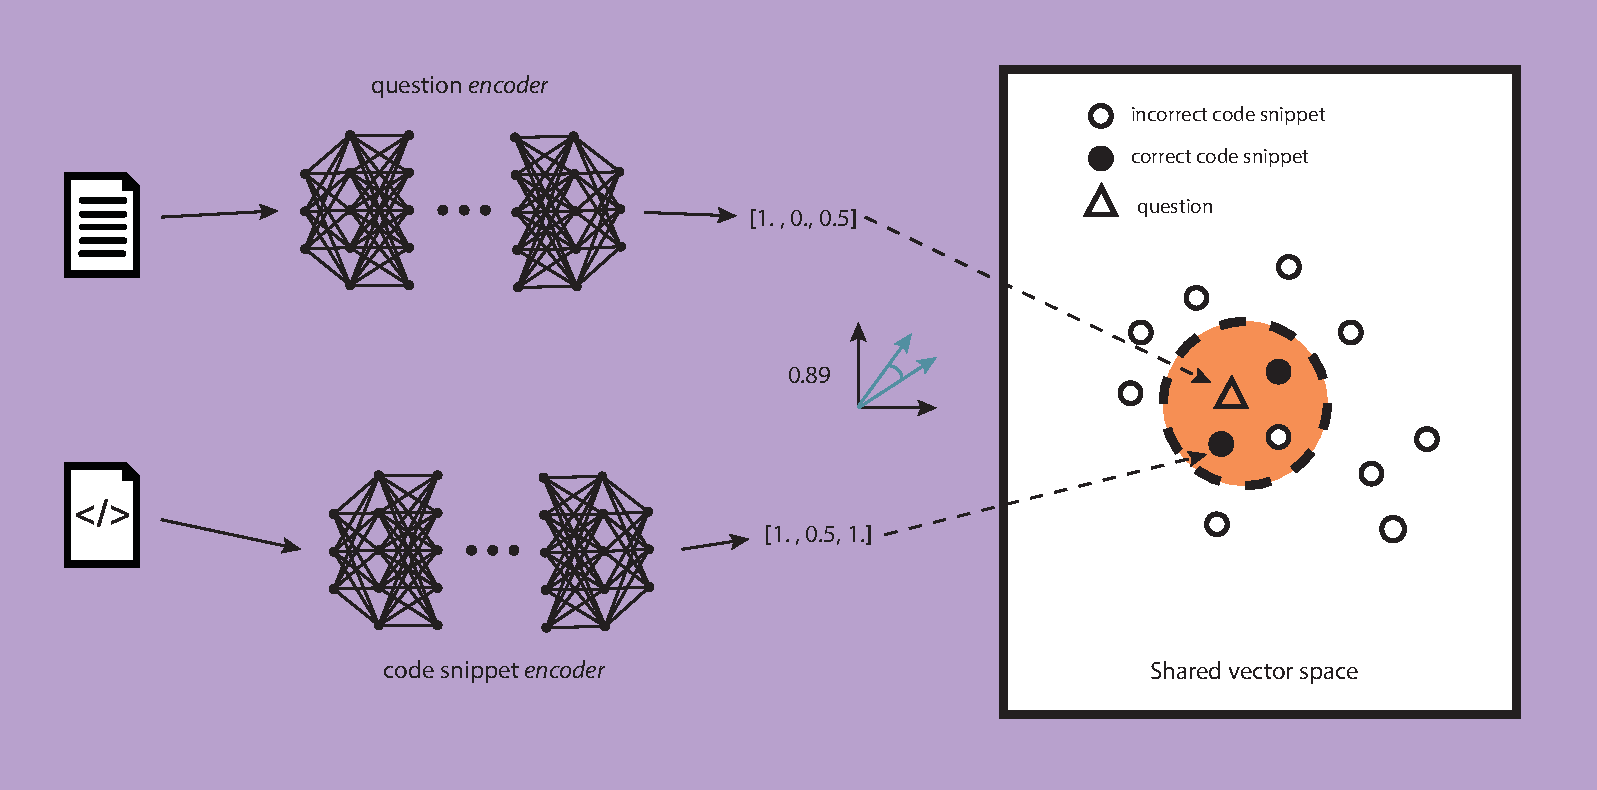
\includegraphics[width=1\textwidth]{resources/joint_embedding-article.pdf}
          \caption{Illustration of joint embedding technique.}
          
          \label{fig:joint-embedding}
        \end{figure}
    \end{frame}
    
    \toclesssection{Methodology}
    
    \begin{frame}{Convolutional neural network}
      \begin{figure}[h]
          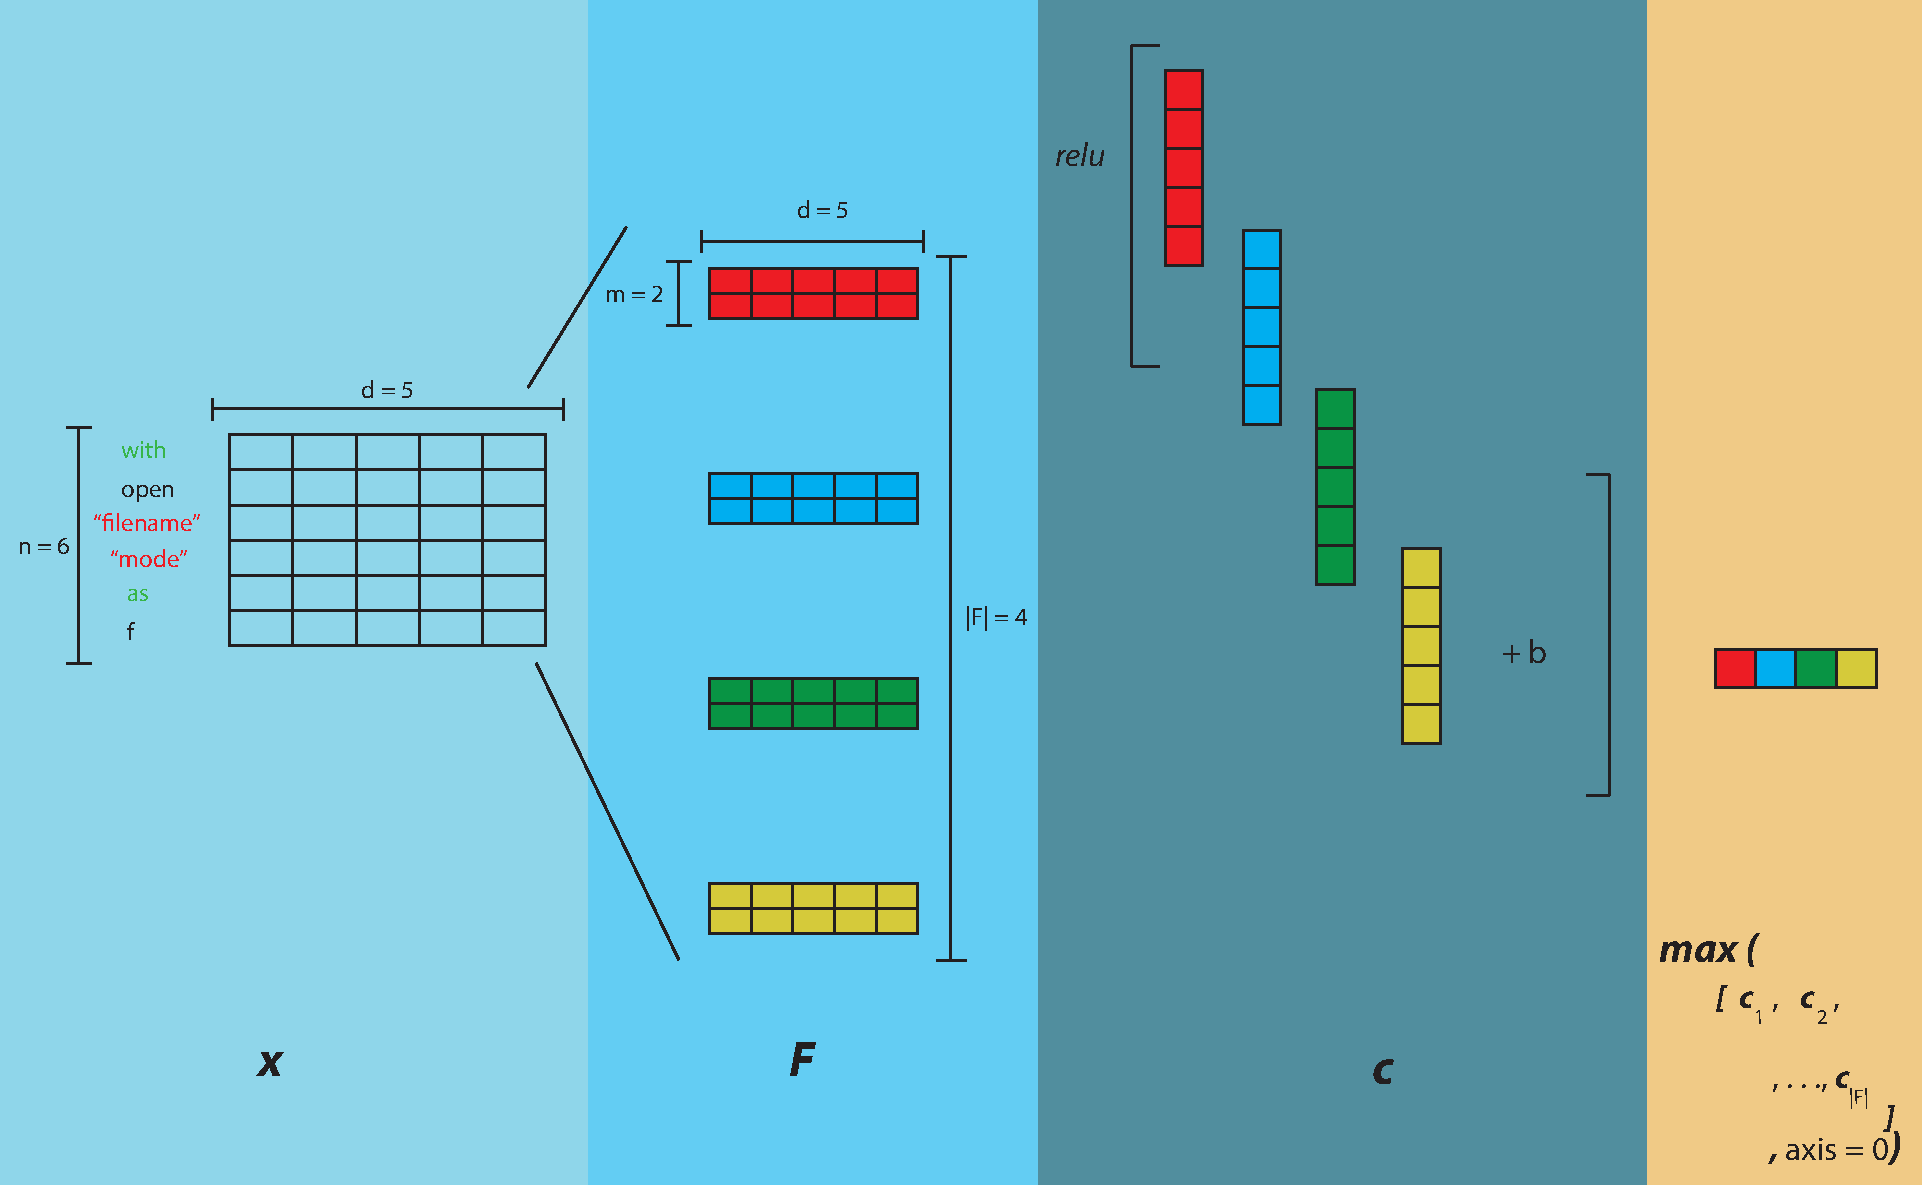
\includegraphics[width=0.85\textwidth]{resources/cnn-steps-word-embedding-article.pdf}
          \caption{Illustration of convolutional neural network steps.}
          
          \label{fig:convolutional-neural-network-steps}
        \end{figure}
    \end{frame}
    
    \toclesssection{Experiments}
    
    \begin{frame}{Dataset}
        \begin{table}[!b]
            {\carlitoTLF % Use monospaced lining figures
        \begin{tabularx}{\textwidth}{Xrr}
            & \multicolumn{2}{c}{\textbf{Question}}\\
            \toprule
          \textbf{Code snippet} & \textbf{Python} & \textbf{SQL}  \\
          \toprule
          
            $N_{1}$: Single code snippet in the answer description & $85.294$ & $75.637$ \\
            
            $N_{2}$: Automatically annotated code snippets & $60.083$ & $41.826$ \\
            
            $N_{3}$: Manually annotated code snippets & $2.169$ & $2.056$  \\
          \bottomrule
          \textbf{Total} & $\bm{147.546}$ & $\bm{119.519}$\\
          \bottomrule
        \end{tabularx}}
        \caption{Summary of StaQC dataset \cite{yao-2018}.}
    \label{table:summary-training-data-yao-staqc}
        \end{table}
        \begin{tikzpicture}[overlay]
\draw[red,ultra thick,rounded corners] (7.4,1.6) rectangle (9.0,5.7);
\end{tikzpicture}
    \end{frame}
    
    \begin{frame}{Evaluation}
      \begin{figure}
          \begin{subfigure}[h]{0.45\textwidth}
            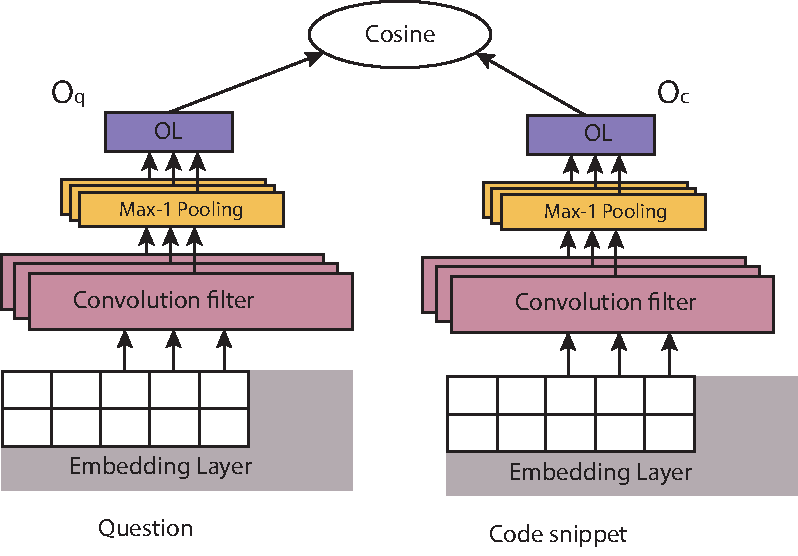
\includegraphics[width=\textwidth]{resources/cnn-architecture-proposal-sbes.pdf}
            \caption{\textit{Our architecture}}
            \label{fig:our-architecture}
          \end{subfigure}
          \hspace{1em}%
          \begin{subfigure}[h]{0.45\textwidth}
            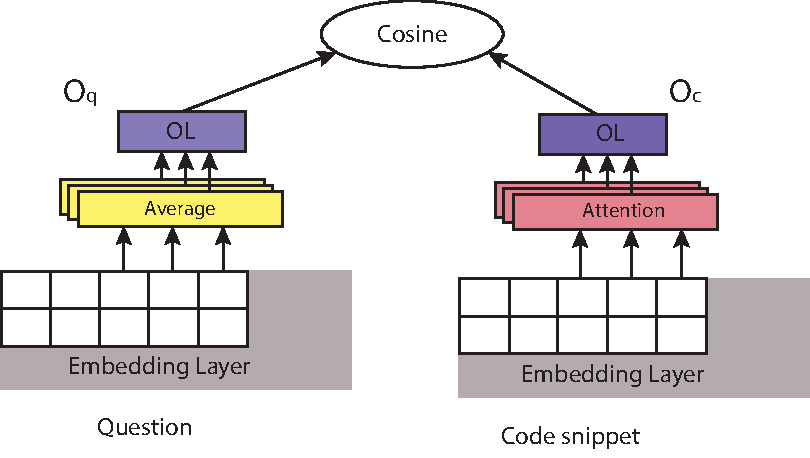
\includegraphics[width=\textwidth]{resources/unif-architecture-sbes.pdf}
            \caption{SOTA architecture}
            \label{fig:unif-architecture}
          \end{subfigure}
          
          \begin{subfigure}[h]{0.45\textwidth}
            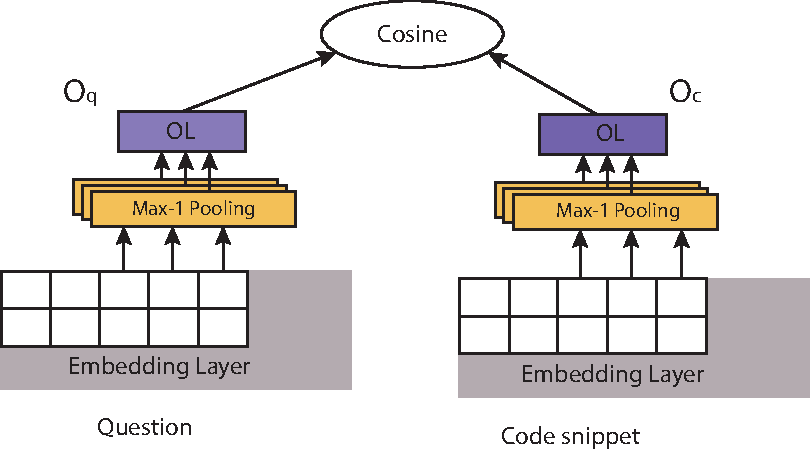
\includegraphics[width=\textwidth]{resources/embedding-architecture-sbes.pdf}
            \caption{Baseline architecture}
            \label{fig:baseline-one-architecture}
          \end{subfigure}
        \end{figure}
    \end{frame}
    \toclesssection{Results}
    \begin{frame}{Results}
    
        \begin{table}[!b]
\footnotesize
\begin{tabularx}{\textwidth}{XXX}
 \toprule
 \textbf{Models} & \textbf{MRR} & \textbf{TOP-1}\\
 \toprule
 Embedding & $0.637$& $0.493 \pm 0.009$\\
 
 \bottomrule
 
 Unif & $0.675 \pm 0.006$ & $0.539 \pm 0.009$\\
 
 \bottomrule
 
\textit{Our model} & $0.701 \pm 0.008$ & $0.577 \pm 0.015$\\
 
\bottomrule
\end{tabularx}
\caption{The experimental results of EVAL sample for Embedding, Unif, and our architecture. }
\label{table:resultados}
\end{table}

        
    \end{frame}
    
    \begin{frame}{Examples}
      \begin{figure}[h]
          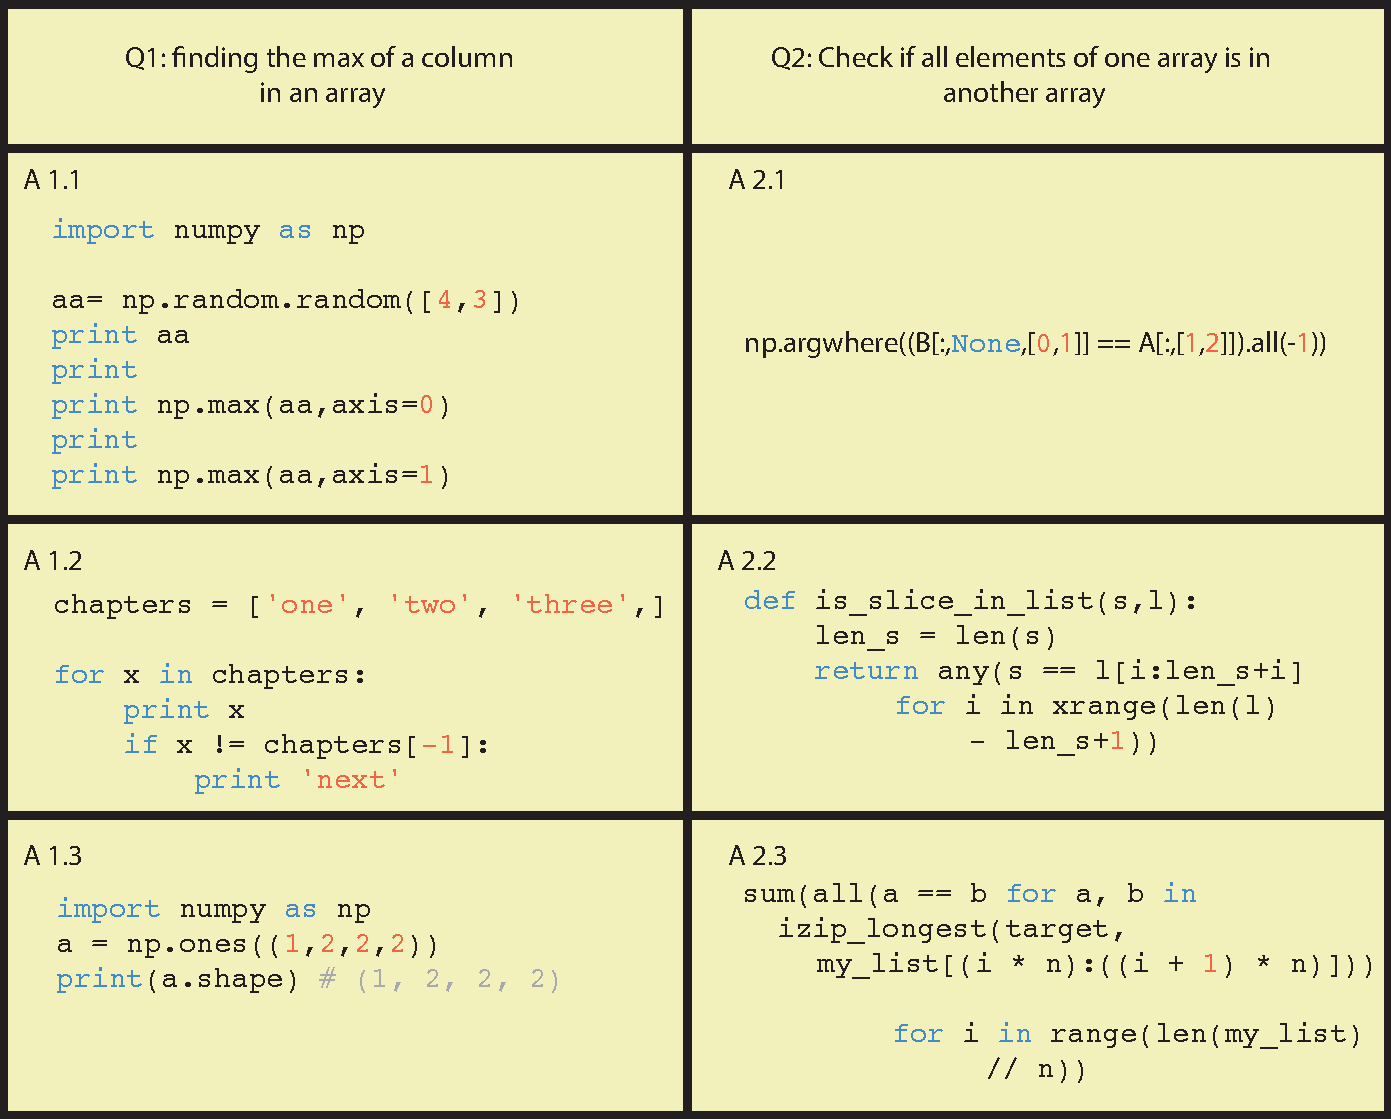
\includegraphics[width=0.75\textwidth]{resources/concrete_examples.pdf}
          \caption{Examples of the output of our tool.}
          
          \label{fig:concrete-examples}
        \end{figure}
    \end{frame}
    
    \toclesssection{Conclusion}
    \begin{frame}{Conclusion}
        Our model achieved:
        \begin{itemize}
            \item TOP-1 accuracy of 60\%, while others achieved 50\%
            \item Top-3 accuracy of 78\%
        \end{itemize}
        Next steps:
        \begin{itemize}
            \item Transfer learning
            \item Pathologies of Neural Models
        \end{itemize}
    \end{frame}
    



\begin{frame}[c]
%\frametitle{A first slide}

\begin{center}
\LARGE Questions?
\end{center}

\end{frame}



    
\appendix
    \begin{frame}[label=bibliography]{Bibliography}
      \bibliographystyle{apalike}
      \bibliography{main}
    \end{frame}

  
\end{document}
